\section{Software Design}
\subsection{Introduction}
The \textit{\textbf{SR2ML}} plug-in scope is mostly to provide a set of capabilities in an integrated system with RAVEN
for probabilistic safety, risk and reliability analysis.
The \textit{\textbf{SR2ML}} plug-in has been coded using the language \emph{Python}. The \emph{Python}
 code can be used as an ``external mode'' in RAVEN (for installation and usage instructions, see~\cite{RAVENuserManual}).
The input of  \textit{\textbf{SR2ML}} is an XML file, which can be read and executed by the plug-in and RAVEN.


\subsection{System Structure (Code)}
\begin{figure}
\centering
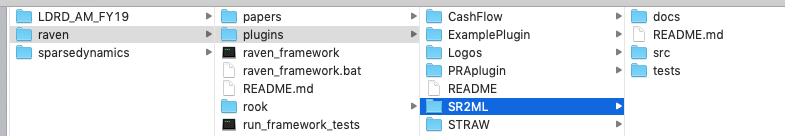
\includegraphics[width=1.0\textwidth]{pics/plugins_location.png}
\caption{Plugins Location}
\label{fig:pluginsLocation}
\end{figure}

The  \textit{\textbf{SR2ML}} plug-in is based on the RAVEN plug-in system. This system is aimed to ease the creation
of external models and modules by external developers without the need to deeply know the internal structure
of the RAVEN software. This system is a transparent API for RAVEN external models.
\\The addition of a plugin does not require modifying RAVEN itself.
Instead, the developer creates a new Python module that is going to be embedded
 in RAVEN at run-time (no need to introduce  hard-coded statements).
 This plugin (SR2ML for instance) needs to be placed in a folder  located in (see figure~\ref{fig:pluginsLocation}):
\begin{lstlisting}[language=bash]
 path/to/raven/plugins/
\end{lstlisting}
In order to install the SR2ML plugin (if not downloaded by RAVEN submodule system),
 the user can run the script contained in the RAVEN script folder:
\begin{lstlisting}[language=bash]
 python path/to/raven/scripts/install_plugins.py  **directory**/SR2ML
\end{lstlisting}
where  $**directory**$/SR2ML should be replaced with the absolute path to the SR2ML plugin directory.
(e.g. ``path/to/my/plugins/SR2ML'').

\subsection{SR2ML Structure}
The  \textit{\textbf{SR2ML}} plug-in contains the following methods (API from RAVEN):

\begin{lstlisting}[language=python]
from ExternalModelPluginBase import ExternalModelPluginBase

class SR2ML(ExternalModelPluginBase):
  def run (self, container, Inputs)
  def _readMoreXML(self, container, xmlNode)
  def initialize(self,container, runInfo, inputs)
\end{lstlisting}
In the following sub-sections all the methods are explained.
\subsubsection{Method: \texttt{run}}
\label{subsubsec:runExternalModelPlugin}
\begin{lstlisting}[language=python]
def run (self, container, Inputs)
\end{lstlisting}

In this function, the SR2ML analysis is coded.
%
The only two attributes this method is going to receive are a Python list of inputs
(the inputs coming from the \texttt{createNewInput} method (see \cite{RAVENuserManual}) and a ``self-like'' object
named ``container''.
%
All the outcomes of the SR2ML module will be stored in the above mentioned ``container'' in order to
allow RAVEN to collect them.

\subsubsection{Method: \texttt{\_readMoreXML}}
\label{subsubsec:externalReadMoreXMLExternalModelPlugin}
\begin{lstlisting}[language=python]
def _readMoreXML(self, container, xmlNode)
\end{lstlisting}
In this method, the SR2ML input is read and made available to the plug-in and RAVEN.
%
The read information are stored in the ``self-like'' object ``container''
 in order to be available to all the other methods, specifically the  \textbf{run} and  \textbf{initialize} methods.
%
The method receives from RAVEN an attribute of type ``xml.etree.ElementTree'',
containing all the sub-nodes and attribute of the XML block \xmlNode{ExternalModel}.
%

Example XML:
\begin{lstlisting}[style=XML,morekeywords={subType,ModuleToLoad}]
  <Models>
    <ExternalModel name="ET" subType="ETModel">
      <variables>statusACC,statusLPI,statusLPR,sequence</variables>
      <!-- xml portion for this plugin only -->
      <map var='statusACC'>ACC</map>
      <map var='statusLPI'>LPI</map>
      <map var='statusLPR'>LPR</map>
      <sequenceID>sequence</sequenceID>
    </ExternalModel>
  </Models>
\end{lstlisting}

\subsubsection{Method: \texttt{initialize}}
\label{subsubsec:externalInitializeExternalModelPlugin}
\begin{lstlisting}[language=python]
def initialize(self, container, runInfo, inputs)
\end{lstlisting}

The \textbf{initialize} method is implemented  to initialize the Cash Flow analysis based on
the current RAVEN status and SR2ML input file (The XML input file).
%
 \\Indeed, RAVEN is going to call this method at the initialization stage of each ``Step'' (see section \cite{RAVENuserManual}).
%
RAVEN will communicate, through a set of method attributes, all the information
that are needed to perform an initialization:
\begin{itemize}
  \item runInfo, a dictionary containing information regarding how the
  calculation is set up (e.g. number of processors, etc.).
  %
  It contains the following attributes:
  \begin{itemize}
    \item \texttt{DefaultInputFile} -- default input file to use
    \item \texttt{SimulationFiles} -- the xml input file
    \item \texttt{ScriptDir} -- the location of the pbs script interfaces
    \item \texttt{FrameworkDir} -- the directory where the framework is located
    \item \texttt{WorkingDir} -- the directory where the framework should be
    running
    \item \texttt{TempWorkingDir} -- the temporary directory where a simulation
    step is run
    \item \texttt{NumMPI} -- the number of mpi process by run
    \item \texttt{NumThreads} -- number of threads by run
    \item \texttt{numProcByRun} -- total number of core used by one run (number
    of threads by number of mpi)
    \item \texttt{batchSize} -- number of contemporaneous runs
    \item \texttt{ParallelCommand} -- the command that should be used to submit
    jobs in parallel (mpi)
    \item \texttt{numNode} -- number of nodes
    \item \texttt{procByNode} -- number of processors by node
    \item \texttt{totalNumCoresUsed} -- total number of cores used by driver
    \item \texttt{queueingSoftware} -- queueing software name
    \item \texttt{stepName} -- the name of the step currently running
    \item \texttt{precommand} -- added to the front of the command that is run
    \item \texttt{postcommand} -- added after the command that is run
    \item \texttt{delSucLogFiles} -- if a simulation (code run) has not failed,
    delete the relative log file (if True)
    \item \texttt{deleteOutExtension} -- if a simulation (code run) has not
    failed, delete the relative output files with the listed extension (comma
    separated list, for example: `e,r,txt')
    \item \texttt{mode} -- running mode, curently the only mode supported is
      mpi (but custom modes can be created)
    \item \textit{expectedTime} -- how long the complete input is expected to
    run
    \item \textit{logfileBuffer} -- logfile buffer size in bytes
  \end{itemize}
  \item inputs, a list of all the inputs that have been specified in the
  ``Step'' using this model.
  %
\end{itemize}
